\subsection*{Task 1}

\subsubsection*{a)}

Intersection over Union (IoU) in the context of object detection is the fraction of area of intersection over area of union between two bounding boxes. \cref{fig:task1:a} displays a typical scenario, where the IoU is found by dividing the sum of pixels that contain the intersection by the sum of pixels that contain the union.

\begin{figure}[h!]
  \centering
  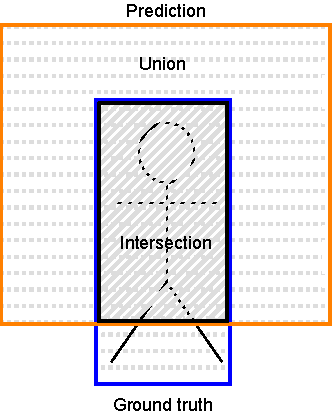
\includegraphics{figures/IoU.pdf}
  \caption{Intersection (dashed) and union (dots) for two bounding boxes when detecting a person from an image.}
  \label{fig:task1:a}
\end{figure}


\subsubsection*{b)}

The equations for precision and recall are

\begin{subequations}
  \begin{align*}
    \text{Precision} &= \frac{\text{TP}}{\text{TP}+\text{FP}}, \\
    \text{Recall} &= \frac{\text{TP}}{\text{TP}+\text{FN}},
  \end{align*}
\end{subequations}

where TP are true positives, FP are false positives and FN are false negatives. A true positive is a correct prediction of a class, while a false positive is an incorrect prediction of a class. In \cref{fig:task1:a}, we have a true positive if we predict there is a person in the image, and a false positive if we predict there is a person in an image when there is not.


\subsubsection*{c)}

The average precision (AP) for each class is

\begin{align*}
  \text{Class 1:}\quad \text{AP}_1 &= \frac{5\cdot 1 + 3\cdot0.5+3\cdot0.2}{11} = 0.645, \\
  \text{Class 2:}\quad \text{AP}_2 &= \frac{4\cdot1 + 1\cdot 0.8 + 1\cdot0.6 +2\cdot0.5+3\cdot0.2}{11} = 0.636.
\end{align*}

The mean average precision (mAP) is then

\begin{equation*}
  \text{mAP} = \frac{1}{K} \sum_{i=1}^K \text{AP}_i = \frac{0.645 + 0.636}{2} = 0.6405. 
\end{equation*}
